\documentclass[25pt, a0paper, portrait, margin=0mm, innermargin=15mm, blockverticalspace=15mm, colspace=15mm, subcolspace=8mm]{tikzposter}

\usepackage{amsmath}
\usepackage{epsf,graphicx,subfig}
\setcounter{tocdepth}{3}
\usepackage{xcolor}
\usepackage{lineno}
\usepackage[nolist]{acronym}
\usepackage{epsf,graphicx,subfig}
\usepackage{amssymb,amsmath}
\usepackage{tikz}
\usetikzlibrary{positioning}
\usepackage{todonotes}
\usepackage{standalone}
\usepackage{scalefnt}
\usepackage{url}

\definecolor{udgColor}{RGB}{82,119,213}


\title{\acs{sift} texture description for understanding breast ultrasound images}
%\author{Joan Massich\inst{1}\inst{2}\thanks{This work was partially supported by the Spanish Science and Innovation grant nb. TIN2012-37171-C02-01 and TTIN2012-37171-C02-02 and the Regional Council of Burgundy.} \and Fabrice Meriaudeau \inst{2} \and Melcior Sent{\'i}s\inst{3} \and Sergi Ganau\inst{3} \and Elsa~P{\'e}rez\inst{4} 
%\and Domenec Puig\inst{5} \and Robert  Mart{\'i} \inst{1} \and  Arnau Oliver\inst{1}\and Joan Mart{\'i} \inst{1}}
%\institute{Computer Vision and Robotics Group, University of Girona, Spain. \email{jmassich@atc.udg.edu} \and
%Laboratoire Le2i-UMR CNRS, University of Burgundy,  Le Creusot, France.
% \and Department of
%Breast and Gynecological Radiology,  UDIAT-Diagnostic Center, Parc
%Taul{\'i} Corporation, Sabadell, Spain.
% \and 
%Department of Radiology, Hospital Josep Trueta of Girona, Spain.
%\and
%Department of Computer Engineering and Mathematics, University Rovira i Virgili, Tarragona, Spain.}

\author{Joan Massich, Fabrice Meriaudeau, Melcior Sent{\'i}s, Sergi Ganau, Elsa~P{\'e}rez, Domenec Puig, Robert  Mart{\'i}, Arnau Oliver and Joan Mart{\'i}}

%\institute{contact author: sik@eia.udg.edu}
%\usetheme{Autumn}\usecolorstyle[colorPalette=BrownBlueOrange]{Germany}
\usetheme{Simple}
%\usecolorstyle[colorOne=udgColor]{Russia} 
\usecolorstyle[colorOne=udgColor]{Denmark} 

% This tex, loads the Breast GT pallete if is not defined.
% The document takes advantage of the xcolor package primitive 
% \def\@ifundefinedcolor#1{\@ifundefined{\string\color@#1}}
% therefore it xcolor package is needed or the definitions needs to be added.
% 
% TODO: 
% 	create a more generic script that checks if all the packages are there otherwise loads them.
%	or defines the missing primitive.
%   take a look at: \@ifpackageloaded{<name>}{<true>}{<false>}
% 					http://tex.stackexchange.com/questions/16199/test-if-a-package-or-package-option-is-loaded

\makeatletter
\newcommand{\colorprovide}[2]{%
  \@ifundefinedcolor{#1}{\colorlet{#1}{#2}}{}}

\newcommand{\defineColorWhenNoExist}[3]{%
  \@ifundefinedcolor{#1}{\definecolor{#1}{#2}{#3}}{}}
\makeatother

\defineColorWhenNoExist{bgColor}{rgb}{0.0000, 0.0000, 0.0000}
\defineColorWhenNoExist{boundaryColor}{rgb}{0.8784, 0.8784, 0.7529}
\defineColorWhenNoExist{chestWallColor}{rgb}{0.5294, 0.7843, 0.6078}
\defineColorWhenNoExist{fatColor}{rgb}{0.9804, 0.5882, 0.1176}
\defineColorWhenNoExist{fibroGlandColor}{rgb}{1.0000, 1.0000, 0.0000}
\defineColorWhenNoExist{lesionColor}{rgb}{1.0000, 0.2510, 0.0000}
\defineColorWhenNoExist{lungColor}{rgb}{0.2353, 0.6078, 0.8235}
\defineColorWhenNoExist{pectoralColor}{rgb}{0.6510, 0.3490, 1.0000}
\defineColorWhenNoExist{ribColor}{rgb}{0.0000, 0.4510, 0.1961}
\defineColorWhenNoExist{skinColor}{rgb}{0.9804, 0.7255, 0.7451}
\defineColorWhenNoExist{unkTissueColor}{rgb}{0.6000, 0.3020, 0.2510}


\begin{document}\maketitle
/home/sik/Work/escola/recerca/iwdm2014/paper/acronyms.tex

\graphicspath{{figures/paperFigures/}}
\acresetall

\block{Abstract}{
Texture is a powerful cue for describing structures that show a high degree of similarity in their image intensity patterns. This paper describes the use of \acf{sift}, both as low-level and high-level descriptors, applied to differentiate the tissues present in breast US images. For the low-level texture descriptors case, \ac{sift} descriptors are extracted from a regular grid. The high-level texture descriptor is build as a \ac{bof} of \ac{sift} descriptors. 
Experimental results are provided showing the validity of the proposed approach for describing the tissues in breast US images.
}
%\begin{keywords}
%breast cancer, ultrasound, texture, SIFT
%\end{keywords}

\begin{columns} \column{0.45}

\block{Problem definition}{
 \begin{tikzfigure}[Dataset sample. From left to right: image sample, accompanying multi-label \ac{gt}, tissue label \ac{gt} color-coding.]
      \centering
%	\documentclass[border=2pt]{standalone}
\usepackage{tikz}
\usepackage{pgfplots,pgfplotstable}
\pgfplotsset{compat=1.8}
\usetikzlibrary{positioning}

\graphicspath{{../paperFigures/}}
% This tex, loads the Breast GT pallete if is not defined.
% The document takes advantage of the xcolor package primitive 
% \def\@ifundefinedcolor#1{\@ifundefined{\string\color@#1}}
% therefore it xcolor package is needed or the definitions needs to be added.
% 
% TODO: 
% 	create a more generic script that checks if all the packages are there otherwise loads them.
%	or defines the missing primitive.
%   take a look at: \@ifpackageloaded{<name>}{<true>}{<false>}
% 					http://tex.stackexchange.com/questions/16199/test-if-a-package-or-package-option-is-loaded

\makeatletter
\newcommand{\colorprovide}[2]{%
  \@ifundefinedcolor{#1}{\colorlet{#1}{#2}}{}}

\newcommand{\defineColorWhenNoExist}[3]{%
  \@ifundefinedcolor{#1}{\definecolor{#1}{#2}{#3}}{}}
\makeatother

\defineColorWhenNoExist{bgColor}{rgb}{0.0000, 0.0000, 0.0000}
\defineColorWhenNoExist{boundaryColor}{rgb}{0.8784, 0.8784, 0.7529}
\defineColorWhenNoExist{chestWallColor}{rgb}{0.5294, 0.7843, 0.6078}
\defineColorWhenNoExist{fatColor}{rgb}{0.9804, 0.5882, 0.1176}
\defineColorWhenNoExist{fibroGlandColor}{rgb}{1.0000, 1.0000, 0.0000}
\defineColorWhenNoExist{lesionColor}{rgb}{1.0000, 0.2510, 0.0000}
\defineColorWhenNoExist{lungColor}{rgb}{0.2353, 0.6078, 0.8235}
\defineColorWhenNoExist{pectoralColor}{rgb}{0.6510, 0.3490, 1.0000}
\defineColorWhenNoExist{ribColor}{rgb}{0.0000, 0.4510, 0.1961}
\defineColorWhenNoExist{skinColor}{rgb}{0.9804, 0.7255, 0.7451}
\defineColorWhenNoExist{unkTissueColor}{rgb}{0.6000, 0.3020, 0.2510}


\begin{document}
\newcommand\mySize{13cm}
% argument #1: any options
\newenvironment{customlegend}[1][]{%
    \begingroup
    % inits/clears the lists (which might be populated from previous
    % axes):
    \csname pgfplots@init@cleared@structures\endcsname
    \pgfplotsset{#1}%
}{%
    % draws the legend:
    \csname pgfplots@createlegend\endcsname
    \endgroup
}%
% makes \addlegendimage available (typically only available within an
% axis environment):
\def\addlegendimage{\csname pgfplots@addlegendimage\endcsname}

\begin{tikzpicture}



\tikzstyle{myLegendStyle} = [ align=left,
                              draw=none,
                              column sep=2ex,
                              font=\tiny,
                            ]

%\newcommand\addMyLegendArea[1][]
%  { \addlegendimage{#1,area legend} }
  
\begin{customlegend}
  [ legend columns=   5,
    legend style  =   myLegendStyle,
    legend entries= { Background,                 
                      Chest wall,        
                      Pectoral muscle,                         
                      Adipose tissue,       
                      Lesion,            
                      Air (or lungs),                   
                      Rib,                            
                      Fibro-glandular tissue,      
                      Skin,                         
                      Boundary,                            
                    },
    anchor = north,
    at = {(0,4)},
  ]

%  \addMyLegendArea{red}
  \addlegendimage{bgColor!50!black,         fill=bgColor,         area legend}
  \addlegendimage{chestWallColor!50!black,  fill=chestWallColor,  area legend}
  \addlegendimage{pectoralColor!50!black,   fill=pectoralColor,   area legend}
  \addlegendimage{fatColor!50!black,        fill=fatColor,        area legend}
  \addlegendimage{lesionColor!50!black,     fill=lesionColor,     area legend}
  \addlegendimage{lungColor!50!black,       fill=lungColor,       area legend}
  \addlegendimage{ribColor!50!black,        fill=ribColor,        area legend}
  \addlegendimage{fibroGlandColor!50!black, fill=fibroGlandColor, area legend}
  \addlegendimage{skinColor!50!black,       fill=skinColor,       area legend}
  \addlegendimage{boundaryColor!50!black,   fill=boundaryColor,   area legend}

\end{customlegend}

\node[anchor=south west,inner sep=0] (imgNode) at (-11.5,1.5) {\includegraphics[width=\mySize]{pngImgs/gt/000002.png}};

\node[anchor=south east,inner sep=0] at (-12,1.5) {\includegraphics[width=\mySize]{pngImgs/000002.png}};

\end{tikzpicture}
\end{document}

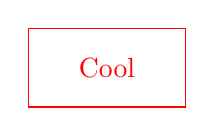
\begin{tikzpicture}
\draw [color=red] (0,0) rectangle (2,1) node [midway] {Cool};
\end{tikzpicture}
\end{tikzfigure}
}


\block{xxxxxxxxxx}{
\begin{tikzfigure}[\acs{sift} space. (a) Projected space colored according to \acs{gt} tissue labeling. (b) $P(\bar{x}_a)$. (c) $P(\omega)$.]
\begin{tikzpicture}


\node[anchor=south east,inner sep=0] (mappedGTNode) at (0,0) {\includegraphics[trim=115 250 118 250,clip,height=.12\textwidth]{mapGTintoSIFT}};

\node[anchor=south west,inner sep=0](occurrenceMap) at (-8pt,0) {\includegraphics[height=.12\textwidth]{siftOccurrences2}};


\definecolor{lungColor}{rgb}{0.2353, 0.6078, 0.8235}
\definecolor{chestWallColor}{rgb}{0.5294, 0.7843, 0.6078}
\definecolor{ribColor}{rgb}{0.0000, 0.4510, 0.1961}
\definecolor{pectoralColor}{rgb}{0.6510, 0.3490, 1.0000}
\definecolor{fibroGlandColor}{rgb}{1.0000, 1.0000, 0.0000}
\definecolor{fatColor}{rgb}{0.9804, 0.5882, 0.1176}
\definecolor{skinColor}{rgb}{0.9804, 0.7255, 0.7451}
\definecolor{unkTissueColor}{rgb}{0.6000, 0.3020, 0.2510}
\definecolor{bgColor}{rgb}{0.0000, 0.0000, 0.0000}
\definecolor{lesionColor}{rgb}{1.0000, 0.2510, 0.0000}
\definecolor{boundaryColor}{rgb}{0.8784, 0.8784, 0.7529}
\tikzset{labelSt/.style=
{anchor=north west,rectangle,
node distance=1.96pt,
scale=.6,
minimum width=1pt,minimum height=1pt,
}}

\node[anchor=south west,inner sep=0, right=of occurrenceMap](imgNode) {\includegraphics[trim = 5 5 18 0, clip,width=.12\textwidth]{classPrior}};

\draw[] (imgNode.south west) +(14pt,3.5pt) node[labelSt, draw=bgColor, fill=bgColor] (bgName) {} ;
\draw[] node[labelSt,draw=lungColor, fill=lungColor,right=of bgName] (lungName) {};
\draw[] node[labelSt, draw=chestWallColor,right=of lungName, fill=chestWallColor] (cwName) {} ;
\draw[] node[labelSt, draw=ribColor, fill=ribColor,right=of cwName] (ribName) {} ;
\draw[] node[labelSt, draw=pectoralColor, fill=pectoralColor,right=of ribName] (pectoralName) {} ;
\draw[] node[labelSt, draw=fibroGlandColor, fill=fibroGlandColor,right=of pectoralName] (fibroGlandName) {} ;
\draw[] node[labelSt, draw=fatColor, fill=fatColor,right=of fibroGlandName] (fatName) {} ;
\draw[] node[labelSt, draw=skinColor, fill=skinColor,right=of fatName] (skinName) {} ;
\draw[] node[labelSt, draw=lesionColor, fill=lesionColor,right=of skinName] (lesionName) {} ;
\draw[] node[labelSt, draw=boundaryColor, fill=boundaryColor,right=of lesionName] (boundaryName) {} ;

\end{tikzpicture}
\end{tikzfigure}
} 




\column{0.45} \block{xxxxxxx}{
\begin{tikzfigure}[Distribution of the \acs{sift} descriptors for some classes in the \ac{gt}.]
 \begin{tikzpicture}
\tikzset{myNode/.style=
{anchor=north west,rectangle,
node distance=5pt,
minimum width=8pt,minimum height=8pt,
inner sep=0,
}}

\node[myNode, label=below:Background] (bgNode) at (0,0) {\includegraphics[width=.1\textwidth]{gtDistro/000.png}};
\node[myNode, right=of bgNode, label=below:Air or lungs] (airNode) {\includegraphics[width=.1\textwidth]{gtDistro/001.png}};
\node[myNode, right=of airNode, label=below:Chest wall] (cwNode) {\includegraphics[width=.1\textwidth]{gtDistro/002.png}};

\node[myNode, right=of cwNode, label=below:Rib] (ribNode) {\includegraphics[width=.1\textwidth]{gtDistro/003.png}};

\node[myNode, below=15pt of bgNode, label=below:Fibro-glandular] (fibNode) {\includegraphics[width=.1\textwidth]{gtDistro/005.png}};

\node[myNode, right=of fibNode, label=below:Adipose tissue] (fatNode) {\includegraphics[width=.1\textwidth]{gtDistro/006.png}};
\node[myNode, right=of fatNode, label=below:Skin layers] (skNode) {\includegraphics[width=.1\textwidth]{gtDistro/007.png}};
\node[myNode, right=of skNode, label=below:Lesion] (lesionNode) {\includegraphics[width=.1\textwidth]{gtDistro/128.png}};

\end{tikzpicture} 
\end{tikzfigure}
}

%\begin{subcolumns} \subcolumn{.45} \block{Subcolumns}{If you...} \subcolumn{.5} \block{}{An example...} \end{subcolumns}
%\block[titlewidthscale=.8,bodywidthscale=.9,titleoffsety=9.5mm,bodyoffsety=9mm]{Changing the Poster’s Appearance}{If the default...}

\block{xxx}{
\begin{tikzfigure}[ Qualitative evaluation of the \ac{map} labeling of the feature space.]

\begin{tikzpicture}
\node[anchor=south west,inner sep=0] (imgNode) at (0,0) {\includegraphics[trim = 91 230 90 230, clip,width=.1\textwidth]{labelingMAP.pdf}};

\node[anchor=south east,inner sep=0] at (-8pt,0) {\includegraphics[trim = 85 230 180 230, clip,width=.1\textwidth]{intensityLabelingMAP.pdf}};
\end{tikzpicture}
\end{tikzfigure}
}

\block{xxx}{
\begin{tikzfigure}[ \acs{sift}-\acs{bof} descriptors qualitative analysis. (Left) image example. (Right) Dictionary representation colored using the location of the keypoint location in fig.\,\ref{fig:siftMapping}a space. (1-8) Occurrence of the dictionary's key-points associated to each region highlighted in the original image.]

 \begin{tikzpicture}
\node[anchor=south west,inner sep=0] (imgNode) at (0,0) {\includegraphics[trim = 91 300 100 242, clip,width=.2\textwidth]{appearance1.pdf}};

\tikzset{nameSt/.style=
{anchor=north west,rectangle,
node distance=10pt,
minimum width=8pt,minimum height=8pt,
inner sep=0,
}}
\begin{tiny}

\draw[] (imgNode.north east) +(5pt,0) node[nameSt, label=below:Codebook] (dictionary) {\includegraphics[width=.10\textwidth,]{dictionary/01.png}} ;
\draw[] (dictionary.north east) +(5pt,0) node[nameSt, label=below:(1)] (BoFi) {\includegraphics[width=.10\textwidth,]{dictionary/01Signatures/127.png}} ;
\draw[] (BoFi.north east) +(5pt,0) node[nameSt, label=below:(2)] (BoFii) {\includegraphics[width=.02\textwidth,]{dictionary/01Signatures/037.png}} ;

\node[nameSt, below=of dictionary, label=below:(3)] (BoFiii) {\includegraphics[width=.02\textwidth,]{dictionary/01Signatures/054.png}} ;
\node[nameSt, below=of BoFi, label=below:(4)] (BoFiv) {\includegraphics[width=.02\textwidth,]{dictionary/01Signatures/118.png}} ;
\node[nameSt, below=of BoFii, label=below:(5)] (BoFv) {\includegraphics[width=.02\textwidth,]{dictionary/01Signatures/160.png}} ;

\node[nameSt, below=of BoFiii, label=below:(6)] (BoFvi) {\includegraphics[width=.02\textwidth,]{dictionary/01Signatures/061.png}} ;
\node[nameSt, below=of BoFiv, label=below:(7)] (BoFvii) {\includegraphics[width=.02\textwidth,]{dictionary/01Signatures/077.png}} ;
\node[nameSt, below=of BoFv, label=below:(8)] (BoFviii) {\includegraphics[width=.02\textwidth,]{dictionary/01Signatures/043.png}} ;

\end{tiny}

\end{tikzpicture}
\end{tikzfigure}
}



\end{columns}
\block[titleoffsety=-1cm,bodyoffsety=-1cm]{Sample document}{This poster...}
%\note[targetoffsetx=24cm, targetoffsety=-9cm,radius=8cm,width=.75\textwidth,innersep=.4cm]{You can...}
\note[targetoffsetx=0cm,targetoffsety=-9cm,radius=8cm,width=.5\textwidth,innersep=.4cm]{You can...}
\end{document}
